% !TEX program = xelatex
\documentclass[10pt,letterpaper,twocolumn]{article}

% === GEOMETRY ===
\usepackage[top=0.75in, bottom=0.75in, left=0.75in, right=0.75in]{geometry}

% === FONTS ===
\usepackage{fontspec}
\usepackage{unicode-math}
\usepackage{xeCJK}
\setCJKmainfont{Droid Sans Fallback}

\setmainfont{Latin Modern Roman}
\setsansfont{Latin Modern Sans}

% Custom AC fonts
\newfontfamily\acbold{ywft-processing-bold}[
  Path=../../system/public/type/webfonts/,
  Extension=.ttf
]
\newfontfamily\aclight{ywft-processing-light}[
  Path=../../system/public/type/webfonts/,
  Extension=.ttf
]
\newfontfamily\kidlispfont{ComicRelief-Regular}[
  Path=../arxiv-kidlisp/fonts/,
  Extension=.ttf
]
\newfontfamily\kidlispbold{ComicRelief-Bold}[
  Path=../arxiv-kidlisp/fonts/,
  Extension=.ttf
]
\setmonofont{Latin Modern Mono}[Scale=0.85]

% === PACKAGES ===
\usepackage{xcolor}
\usepackage{titlesec}
\usepackage{enumitem}
\usepackage{booktabs}
\usepackage{tabularx}
\usepackage{fancyhdr}
\usepackage{hyperref}
\usepackage{graphicx}
\graphicspath{{figures/}{../arxiv-kidlisp/figures/}}
\usepackage{ragged2e}
\usepackage{microtype}
\usepackage{listings}
\usepackage{natbib}
\usepackage[colorspec=0.92]{draftwatermark}

% === COLORS (AC palette) ===
\definecolor{acpink}{RGB}{180,72,135}
\definecolor{acpurple}{RGB}{120,80,180}
\definecolor{acdark}{RGB}{64,56,74}
\definecolor{acgray}{RGB}{119,119,119}
\definecolor{klbrand}{RGB}{205,92,155}
\definecolor{klcyan}{RGB}{112,214,255}
\definecolor{kldark}{RGB}{48,43,58}
\definecolor{draftcolor}{RGB}{205,92,155}

% === DRAFT WATERMARK ===
\DraftwatermarkOptions{
  text=工作草稿,
  fontsize=3cm,
  color=draftcolor!18,
  angle=45,
  pos={0.5\paperwidth, 0.5\paperheight}
}

% === KIDLISP SYNTAX COLORS ===
\definecolor{klfn}{RGB}{0,136,170}
\definecolor{klform}{RGB}{119,51,170}
\definecolor{klrepeat}{RGB}{170,0,170}
\definecolor{klnum}{RGB}{204,0,102}
\definecolor{klstr}{RGB}{170,120,0}
\definecolor{klcmt}{RGB}{102,102,102}
\definecolor{klmath}{RGB}{0,136,0}
\definecolor{klvar}{RGB}{204,102,0}
\definecolor{klembed}{RGB}{0,136,0}

% KidLisp inline color macros
\newcommand{\kn}[1]{\textcolor{klnum}{#1}}
\newcommand{\kt}[1]{\textcolor{klstr}{#1}}
\newcommand{\kv}[1]{\textcolor{klvar}{#1}}
\newcommand{\ke}[1]{\textcolor{klembed}{\textbf{#1}}}
\newcommand{\km}[1]{\textcolor{klmath}{#1}}

% === HYPERREF ===
\hypersetup{
  colorlinks=true,
  linkcolor=acpurple,
  urlcolor=acpurple,
  citecolor=acpurple,
  pdfauthor={@jeffrey},
  pdftitle={KidLisp 卡片：一张卡片装得下的程序},
}

% === SECTION FORMATTING ===
\titleformat{\section}
  {\normalfont\bfseries\normalsize\uppercase}
  {\thesection.}
  {0.5em}
  {}
\titlespacing{\section}{0pt}{1.2em}{0.3em}

\titleformat{\subsection}
  {\normalfont\bfseries\small}
  {\thesubsection}
  {0.5em}
  {}
\titlespacing{\subsection}{0pt}{0.8em}{0.2em}

% === HEADER/FOOTER ===
\pagestyle{fancy}
\fancyhf{}
\renewcommand{\headrulewidth}{0pt}
\fancyhead[C]{\footnotesize\color{acpink}\textit{工作草稿 --- 请勿引用}}
\fancyfoot[C]{\footnotesize\thepage}

% === CUSTOM COMMANDS ===
\newcommand{\acdot}{{\color{acpink}.}}
\newcommand{\kidlisp}{\textsc{KidLisp}}

% === LISTINGS ===
\lstdefinelanguage{kidlisp}{
  morekeywords=[1]{wipe,ink,line,box,circle,tri,plot,flood,shape,zoom,scroll,spin,blur,contrast,embed,layer,width,height,frame,time,wiggle,melody,mic,suck,sort,form,trans,cube,move,scale,hop,overtone,resolution,write,text,type,stamp,paste,point,poly,noise,fade,pan,unpan,mask,unmask,flip,crawl,left,right,up,down,goto,face,outline,fill,stroke},
  morekeywords=[2]{def,let,if,cond,once,later,lambda,do},
  morekeywords=[3]{repeat},
  morekeywords=[4]{random,sin,cos,tan,floor,ceil,round,abs,sqrt,min,max},
  sensitive=true,
  morecomment=[l]{;},
  morestring=[b]",
  escapeinside={|}{|},
}
\lstset{
  language=kidlisp,
  basicstyle=\ttfamily\small,
  keywordstyle=[1]\color{klfn}\bfseries,
  keywordstyle=[2]\color{klform}\bfseries,
  keywordstyle=[3]\color{klrepeat}\bfseries,
  keywordstyle=[4]\color{klmath},
  commentstyle=\color{klcmt}\itshape,
  stringstyle=\color{klstr},
  breaklines=true,
  frame=single,
  rulecolor=\color{acgray!30},
  backgroundcolor=\color{acgray!5},
  xleftmargin=0.5em,
  xrightmargin=0.5em,
  aboveskip=0.5em,
  belowskip=0.5em,
}

\lstdefinelanguage{python}{
  morekeywords={def,return,import,from,class,if,else,for,in,with,as,try,except,None,True,False,self,and,or,not,lambda,yield,pass,break,continue,raise,while},
  sensitive=true,
  morecomment=[l]{\#},
  morestring=[b]",
  morestring=[b]',
}
\lstset{
  language=kidlisp,
}

% === LIST SETTINGS ===
\setlist[itemize]{nosep, leftmargin=1.2em, itemsep=0.1em}
\setlist[enumerate]{nosep, leftmargin=1.2em}

% === COLUMN SEPARATION ===
\setlength{\columnsep}{1.8em}

% === PARAGRAPH SETTINGS ===
\setlength{\parindent}{1em}
\setlength{\parskip}{0.3em}

\tolerance=800
\emergencystretch=1em
\hyphenpenalty=50

\begin{document}

% ============ TITLE BLOCK ============

\twocolumn[{%
\begin{center}

\includegraphics[height=4em]{pals}\par\vspace{0.5em}
{\kidlispbold\fontsize{24pt}{28pt}\selectfont\color{kldark} Kid{\color{klbrand}Lisp} 卡片}\par
\vspace{0.2em}
{\kidlispfont\fontsize{11pt}{13pt}\selectfont\color{klbrand} 一张卡片装得下的程序}\par
\vspace{0.6em}
{\normalsize\href{https://prompt.ac/@jeffrey}{@jeffrey}}\par
{\small\color{acgray} Aesthetic\acdot Computer}\par
{\small\color{acgray} ORCID: \href{https://orcid.org/0009-0007-4460-4913}{0009-0007-4460-4913}}\par
\vspace{0.3em}
{\small\color{acpurple} \url{https://kidlisp.com} \enspace$\cdot$\enspace \url{https://aesthetic.computer}}\par
\vspace{0.6em}
\rule{\textwidth}{1.5pt}
\vspace{0.5em}
\end{center}

\begin{center}
{\small\color{acpink}\textbf{[ 工作草稿 --- 请勿引用 ]}}
\end{center}
\vspace{0.3em}

\begin{quote}
\small\noindent\textbf{摘要。}
\kidlisp{} 程序很短。一个典型的程序只有2--4行S-表达式，即可产生一幅完整的视觉构图------一个星芒、一条螺旋、一幅拼布、一个分形。这种简短不是偶然的，而是刻意设计的：该语言省略了用户定义函数、递归和抽象机制，因此程序保持扁平且可读。我们观察到，这种扁平性在程序与物理卡片之间创造了一种自然的对应关系。一个 \kidlisp{} 程序、其源代码和渲染输出可以共存于一张印刷卡片上。本文描述了 \emph{KidLisp Cards} 格式------一组按视觉类别组织的程序卡牌------以及一个 Python 渲染管线（基于 PIL 的解释器），可在浏览器外生成卡片图像。我们讨论了卡片目前是什么（一本精心策划的视觉公案笔记本）、它们可能成为什么（集换卡、教学序列、印刷乐谱、邮寄艺术），以及卡片约束如何反馈到语言设计中。
\end{quote}
\vspace{0.5em}
}]

% ============ 1. 引言 ============

\section{引言}

大多数编程语言产生的程序太长，无法打印在一张索引卡上。这是抽象的结果：通用编程语言鼓励将程序分解为函数、类、模块和文件。程序分散在整个代码库中。没有单一的制品能够捕捉全貌。

\kidlisp{} 不同。它的程序通常只有1--6行。一个完整的动画场景、一个几何图案、一个递归分形或一个莫尔干涉图案只需几个S-表达式。这不是一种限制，而是一种设计选择：\kidlisp{} 省略了用户定义函数、递归（除了通过 \texttt{later}）、可变数据结构和导入。程序是绘图命令、循环和条件的扁平序列。

这种扁平性创造了一个机会。如果一个程序的源代码能放在一张卡片上，而该程序的视觉输出也能放在同一张卡片上，那么卡片就成为一个自包含的制品：一个你可以拿在手中、递给别人、钉在墙上或邮寄的程序。卡片既是文档又是可执行的。它是一份\emph{乐谱}------产生视觉事件的指令。

本文描述了 KidLisp Cards 格式（\S\ref{sec:format}）、离线渲染管线（\S\ref{sec:pipeline}）、当前卡片目录（\S\ref{sec:catalog}）、布局变体及其社会和物理可供性（\S\ref{sec:layouts}），以及该格式的推测性未来（\S\ref{sec:futures}）。

% ============ 2. 卡片格式 ============

\section{卡片格式}
\label{sec:format}

一张 KidLisp 卡片有三个元素：

\begin{enumerate}
  \item \textbf{标题。}一个简短的名称，唤起视觉输出的意象：``Starburst''、``Honeycomb''、``Spiral Walk''。
  \item \textbf{渲染输出。}一张像素艺术图像（默认分辨率160$\times$120，使用最近邻插值3$\times$放大以保持锐利边缘）。
  \item \textbf{源代码。}完整的 \kidlisp{} 程序，通常1--4行，以等宽字体显示在图像下方。
\end{enumerate}

卡片是自包含的：任何阅读源代码的人都可以在任何 \kidlisp{} 解释器中精确复现图像。没有外部依赖，没有导入，没有配置。程序\emph{就是}卡片。

\subsection{卡片尺寸}

渲染图像占据160$\times$120像素的画布（4:3比例），与 \kidlisp{} 的默认分辨率一致。在3$\times$放大时，产生480$\times$360像素的图像，适合屏幕显示。用于打印时，卡片尺寸为4$\times$6英寸（标准索引卡/明信片），图像占据上部，源代码在下方。

\subsection{什么构成好卡片}

不是每个 \kidlisp{} 程序都能成为好卡片。最好的卡片共享以下特征：

\begin{itemize}
  \item \textbf{简短。}1--4行。如果源代码不能舒适地放在图像下方，程序对这种格式来说就太长了。
  \item \textbf{惊喜。}输出应该比源代码所暗示的更复杂或更美丽。一个产生莫尔图案的三行程序值得仔细审视。
  \item \textbf{可读性。}读者应该能够在不运行程序的情况下从源代码追踪到输出。代码和图像之间的联系应该是可辨识的，即使不是立即显而易见的。
  \item \textbf{独立性。}没有 \texttt{\$code} 嵌入，没有外部状态。卡片必须独立运行。
\end{itemize}

\begin{figure}[t]
\centering
\fbox{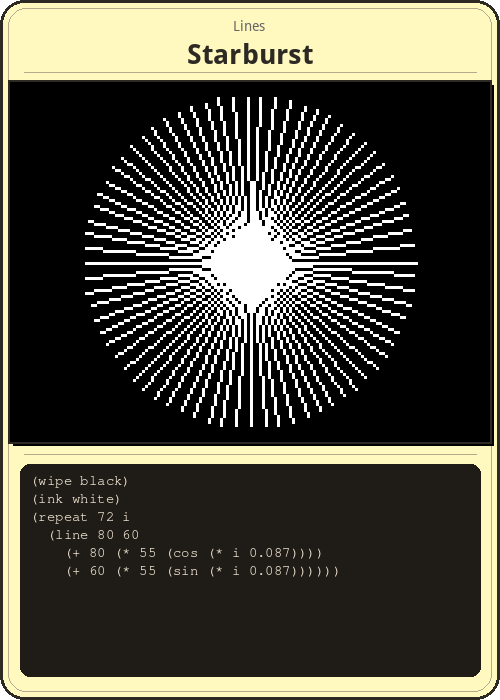
\includegraphics[width=0.47\columnwidth]{card-starburst.png}}%
\hfill%
\fbox{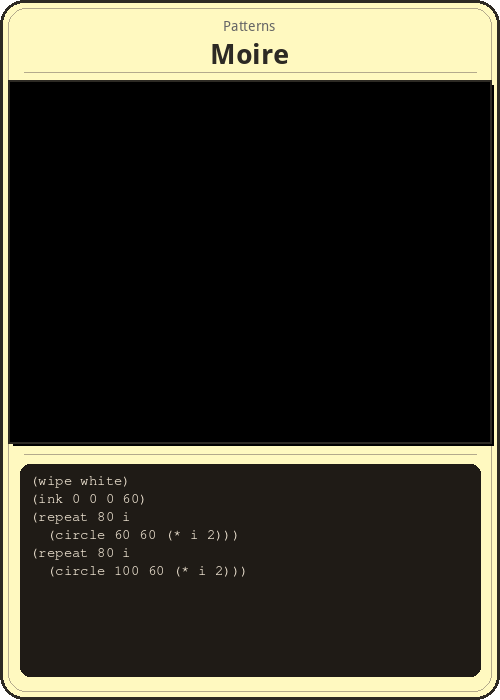
\includegraphics[width=0.47\columnwidth]{card-moire.png}}
\caption{Python 解释器渲染的两张程序卡片：``Starburst''（72条径向线，3行代码）和``Moir\'{e}''（重叠的同心圆，3行）。这些是简单的示例------它们展示了卡片格式的结构，但并不代表语言的表达范围或格式的雄心。}
\label{fig:program-cards}
\end{figure}

% ============ 3. 渲染管线 ============

\section{离线渲染管线}
\label{sec:pipeline}

KidLisp 卡片使用在浏览器外运行的 Python 解释器进行渲染。这使得批量渲染、印刷制作和基于笔记本的策展成为可能，而无需完整的 Aesthetic\acdot Computer 运行时。

\subsection{Python 解释器}

解释器（\texttt{notebooks/ac.py}，452行）实现了 \kidlisp{} 的一个子集，足以进行静态卡片渲染：

\begin{itemize}
  \item \textbf{绘图：} \texttt{wipe}、\texttt{ink}、\texttt{line}、\texttt{box}、\texttt{circle}、\texttt{tri}、\texttt{plot}、\texttt{shape}、\texttt{flood}
  \item \textbf{海龟：} \texttt{crawl}、\texttt{left}、\texttt{right}、\texttt{goto}、\texttt{face}、\texttt{up}、\texttt{down}
  \item \textbf{控制：} \texttt{repeat}、\texttt{if}、\texttt{def}、\texttt{later}、\texttt{do}
  \item \textbf{数学：}完整的算术、三角函数、\texttt{abs}、\texttt{sqrt}、\texttt{min}、\texttt{max}
  \item \textbf{画布：} \texttt{resolution}、\texttt{fill}、\texttt{outline}、\texttt{stroke}
\end{itemize}

解释器使用 PIL（Pillow）进行渲染。每张卡片在 RGBA 画布上绘制，使用最近邻插值放大，并导出为 PNG。Python 实现有意比浏览器评估器（15,161行）更简单------它省略了动画、音频、嵌入和定时语法，仅专注于静态视觉输出所需的子集。

\subsection{Jupyter Notebook 工作流}

主要的策展工具是一个 Jupyter 笔记本（\texttt{notebooks/kidlisp-cards.ipynb}）。\texttt{show\_card()} 函数渲染程序并将其作为 HTML 卡片内联显示：

\begin{lstlisting}[language=python,basicstyle=\ttfamily\footnotesize]
show_card("Starburst", """(wipe black)
(ink white)
(repeat 72 i
  (line 80 60
    (+ 80 (* 55 (cos (* i 0.087))))
    (+ 60 (* 55 (sin (* i 0.087))))))""")
\end{lstlisting}

每次调用都会生成一张深色背景的卡片，内联显示标题、渲染图像和源代码。笔记本既是开发环境又是画廊------滚动浏览笔记本就像翻阅一副卡牌。

\subsection{两个解释器，一种语言}

两个独立解释器（浏览器中的 JavaScript、笔记本中的 Python）的存在起到了交叉验证的作用。如果一个程序在两者中渲染结果相同，则其行为完全由语言语义而非实现细节决定。依赖浏览器特定功能（动画、音频、嵌入层）的程序在构造上被排除在卡片格式之外------它们在 Python 解释器中根本无法渲染。

% ============ 4. 卡片目录 ============

\section{卡片目录}
\label{sec:catalog}

当前笔记本包含28张卡片，分为七个类别。每个类别通过最小示例探索语言的不同方面。这些程序是刻意选择的简单练习------绘图练习、数学插图、海龟漫步。它们建立了卡片格式的结构，但并不代表其表达潜力。有趣的卡片尚未制作。格式的价值将从那些用简短来表达值得表达之事的程序中涌现，而不是从几何演示中。

\subsection{线条}

线条卡片演示 \texttt{repeat} 和三角函数。一个星芒从中心辐射72条线。一个交叉阴影以低透明度叠加水平和垂直网格。

\begin{figure}[h]
\centering
\fbox{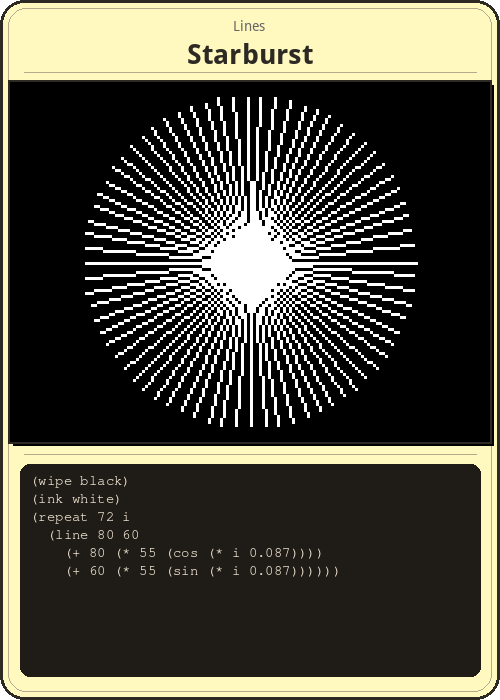
\includegraphics[width=0.47\columnwidth]{card-starburst.png}}%
\hfill%
\fbox{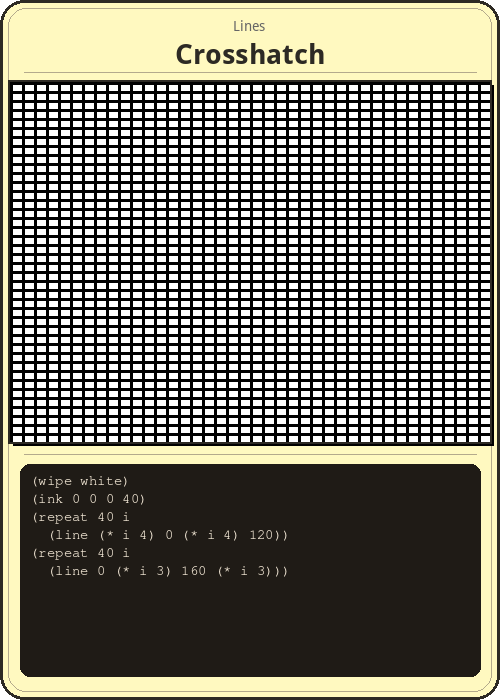
\includegraphics[width=0.47\columnwidth]{card-crosshatch.png}}
\caption{``Starburst'' 和 ``Crosshatch'' --- 线条卡片。}
\label{fig:lines}
\end{figure}

\begin{lstlisting}
; Starburst — 72 radial lines
(wipe |\kt{black}|)
(ink |\kt{white}|)
(repeat |\kn{72}| |\kv{i}|
  (line |\kn{80}| |\kn{60}|
    (|\km{+}| |\kn{80}| (|\km{*}| |\kn{55}| (|\km{cos}| (|\km{*}| |\kv{i}| |\kn{0.087}|))))
    (|\km{+}| |\kn{60}| (|\km{*}| |\kn{55}| (|\km{sin}| (|\km{*}| |\kv{i}| |\kn{0.087}|))))))
\end{lstlisting}

\subsection{圆形}

圆形卡片使用 \texttt{outline} 模式和嵌套 \texttt{repeat} 循环。``Ripple'' 绘制30个同心圆，颜色向蓝色渐变。

\begin{figure}[h]
\centering
\fbox{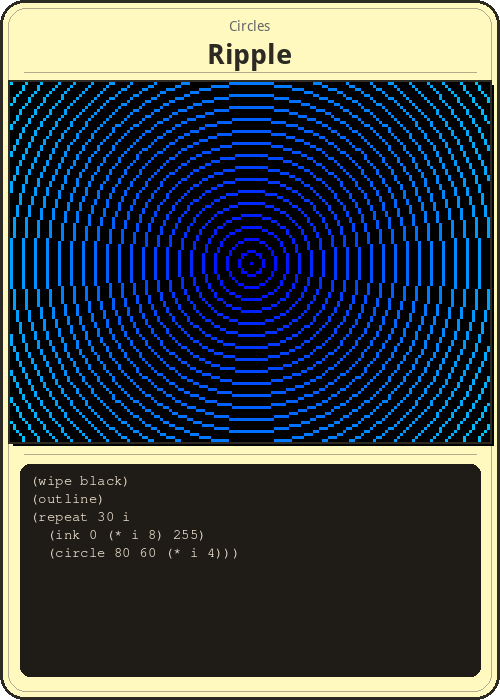
\includegraphics[width=0.47\columnwidth]{card-ripple.png}}%
\hfill%
\fbox{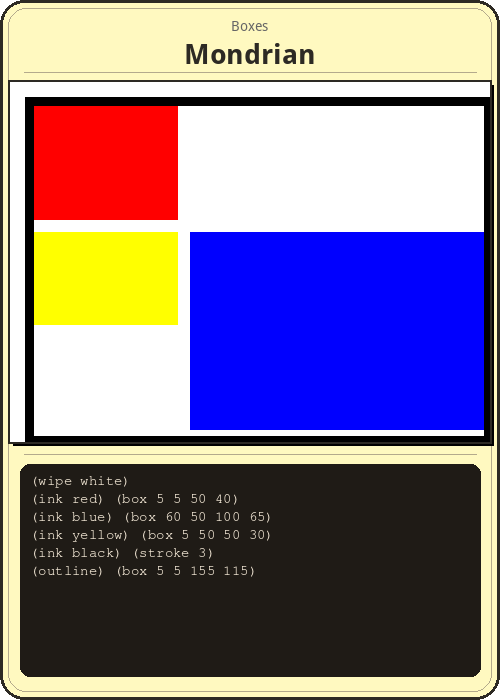
\includegraphics[width=0.47\columnwidth]{card-mondrian.png}}
\caption{``Ripple''（圆形）和 ``Mondrian''（方块）。}
\label{fig:circles-boxes}
\end{figure}

\subsection{方块与构图}

``Mondrian'' 用四个彩色矩形重现原色网格。``Nest'' 绘制10个内嵌矩形，色调逐渐变化。

\subsection{数学与曲线}

这些卡片使用 \texttt{plot} 与数学函数。``Lissajous'' 用600个点绘制利萨如图形。``Spiral'' 绘制极坐标螺旋线。

\begin{figure}[h]
\centering
\fbox{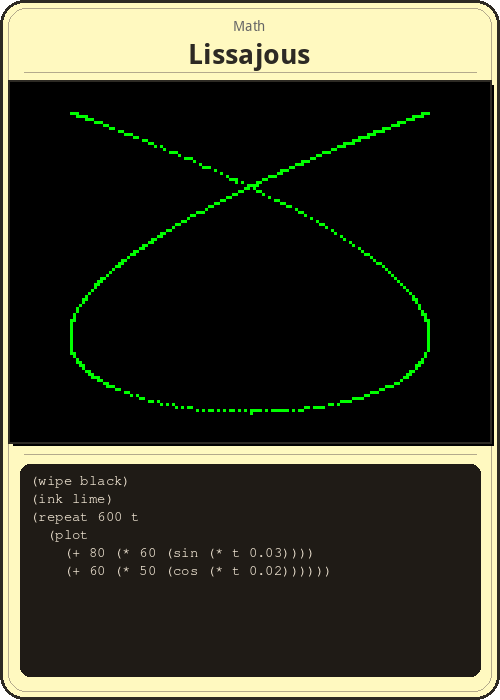
\includegraphics[width=0.47\columnwidth]{card-lissajous.png}}%
\hfill%
\fbox{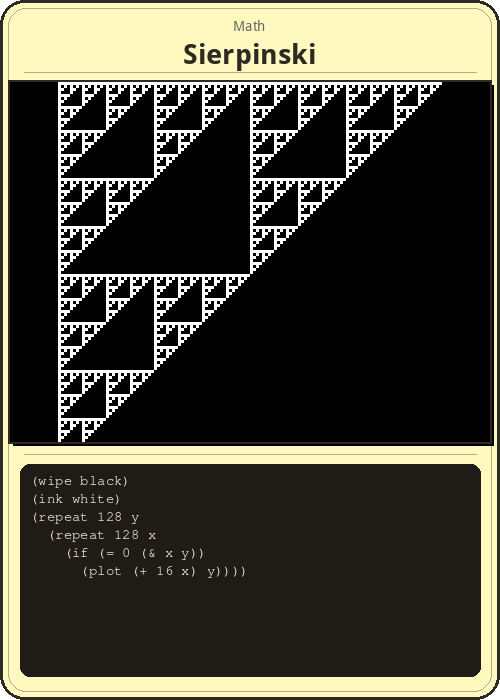
\includegraphics[width=0.47\columnwidth]{card-sierpinski.png}}
\caption{``Lissajous''（数学曲线）和 ``Sierpinski''（位与分形）。}
\label{fig:math}
\end{figure}

\subsection{颜色与渐变}

``Sierpinski'' 使用位与运算生成谢尔宾斯基三角形：\texttt{(if (= 0 (\& x y)) (plot (+ 16 x) y))}。``Sunflower'' 沿黄金角螺旋绘制500个点，颜色循环变化。

\subsection{海龟图形}

海龟卡片使用 \texttt{crawl}、\texttt{left}、\texttt{right} 和 \texttt{face}。一个五角星使用 \texttt{(right 144)}。一棵树使用 \texttt{later} 进行递归分支。一片雪花嵌套科赫曲线段。

\begin{figure}[h]
\centering
\fbox{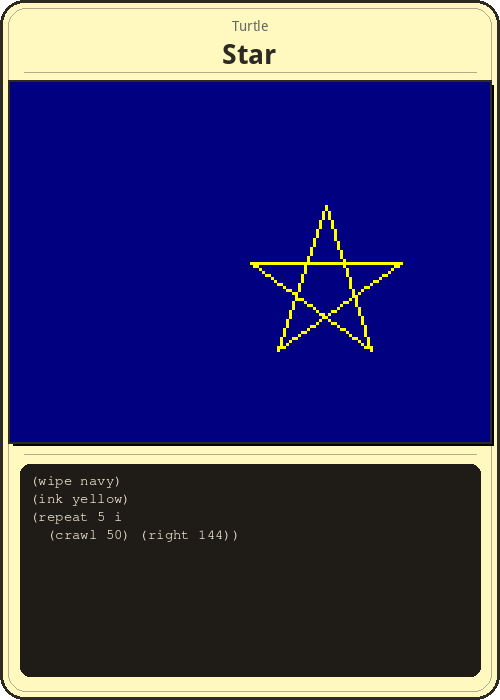
\includegraphics[width=0.47\columnwidth]{card-star.png}}%
\hfill%
\fbox{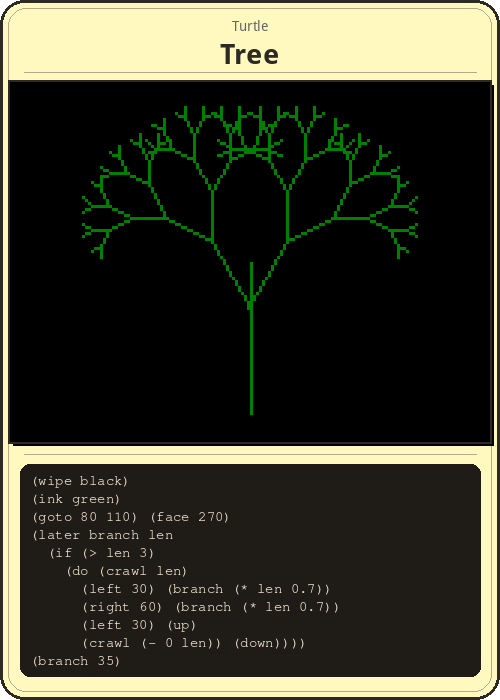
\includegraphics[width=0.47\columnwidth]{card-tree.png}}
\caption{``Star'' 和 ``Tree'' --- 海龟图形卡片。}
\label{fig:turtle}
\end{figure}

\begin{lstlisting}
; Star — 5 sides, 144-degree turns
(wipe |\kt{navy}|)
(ink |\kt{yellow}|)
(repeat |\kn{5}| |\kv{i}| (crawl |\kn{50}|) (right |\kn{144}|))
\end{lstlisting}

\subsection{极简公案}

卡组中最短的卡片。``Horizon'' 是三行：深色天空，金色大地。``Pip'' 是黑色上的一个红点。这些卡片接近最小可行程序------产生可识别图像所需的最少代码量。

\begin{figure}[h]
\centering
\fbox{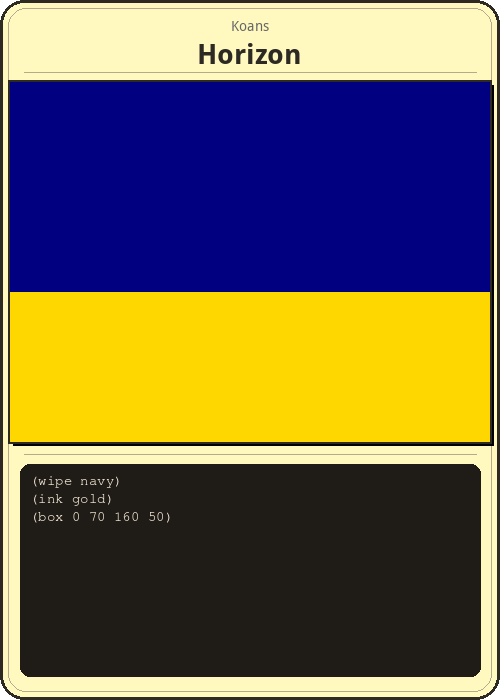
\includegraphics[width=0.47\columnwidth]{card-horizon.png}}%
\hfill%
\fbox{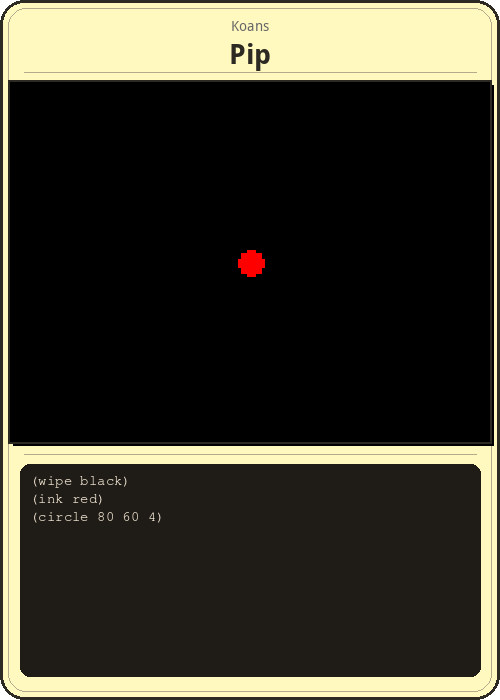
\includegraphics[width=0.47\columnwidth]{card-pip.png}}
\caption{``Horizon'' 和 ``Pip'' --- 极简公案（各2--3行）。}
\label{fig:koans}
\end{figure}

\begin{lstlisting}
; Pip — the minimum card
(wipe |\kt{black}|)
(ink |\kt{red}|)
(circle |\kn{80}| |\kn{60}| |\kn{4}|)
\end{lstlisting}

\begin{figure*}[t]
\centering
\fbox{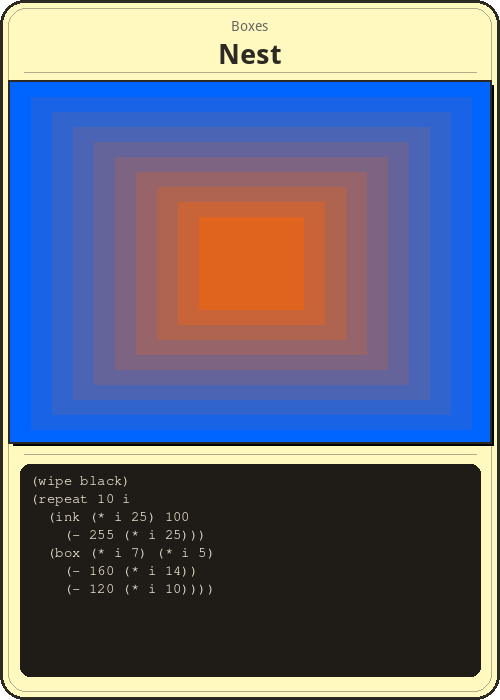
\includegraphics[height=5.5cm]{card-nest.png}}%
\hfill%
\fbox{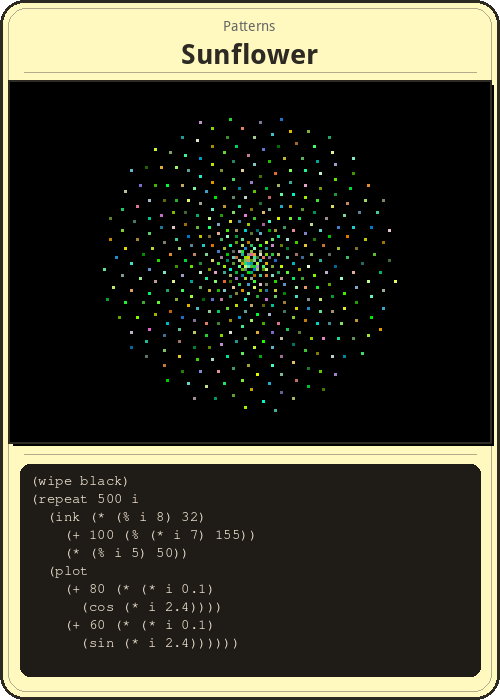
\includegraphics[height=5.5cm]{card-sunflower.png}}%
\hfill%
\fbox{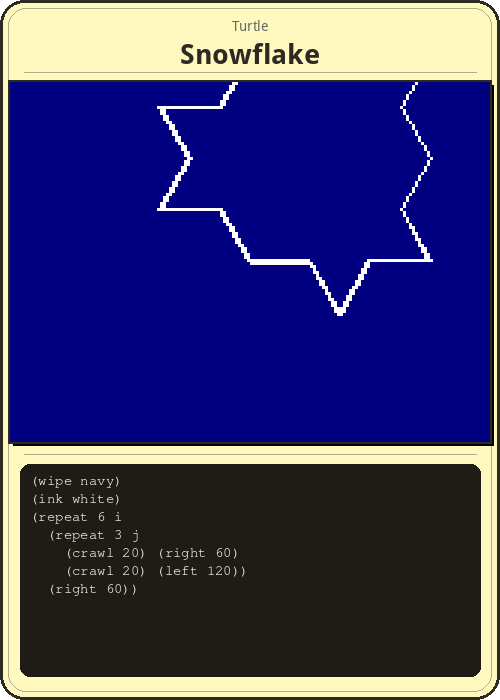
\includegraphics[height=5.5cm]{card-snowflake.png}}%
\hfill%
\fbox{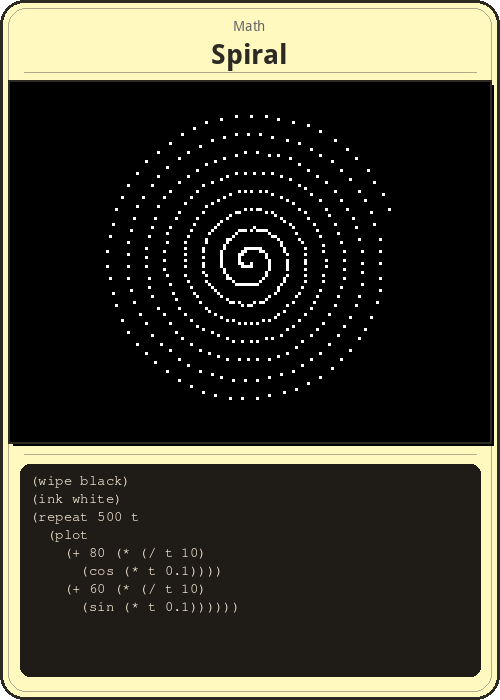
\includegraphics[height=5.5cm]{card-spiral.png}}
\caption{四张完整卡片展示格式：标题、渲染输出和源代码。从左到右：``Nest''、``Sunflower''、``Snowflake''、``Spiral''。每张卡片都是自包含的------图像下方的源代码就是完整程序。这些是简单的绘图练习，而非格式潜力的表达。}
\label{fig:four-cards}
\end{figure*}

% ============ 5. 布局 ============

\section{布局}
\label{sec:layouts}

卡片格式没有固定布局。三个元素（标题、输出、源代码）的排列方式决定了卡片的可供性------你可以用它在物理上和社会上做什么。本节探讨布局变体及其后果。

\begin{figure*}[t]
\centering
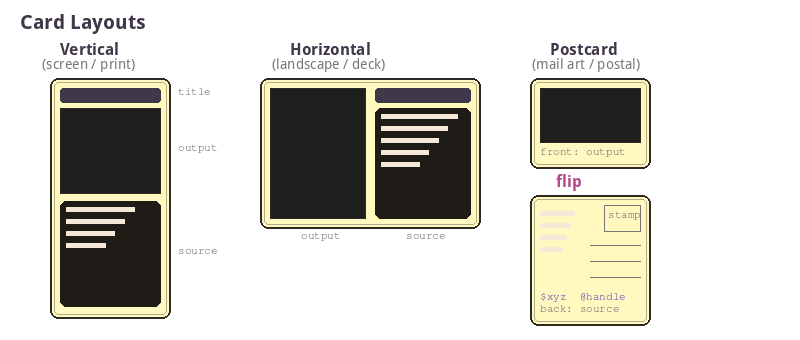
\includegraphics[width=\textwidth]{layout-comparison.png}
\caption{三种布局策略。\textbf{纵向：}标题/图像/源代码从上到下堆叠，针对手机屏幕和纵向打印优化。\textbf{横向：}图像在左，标题和源代码在右，适合横向卡片和并排浏览。\textbf{明信片：}正面是渲染输出，背面是源代码和元数据------一张可邮寄的卡片，翻转后才能看到程序。}
\label{fig:layouts}
\end{figure*}

\subsection{纵向（屏幕/打印）}

默认布局将标题、图像和源代码从上到下堆叠。这是笔记本布局------在手机或 Jupyter 笔记本中自然滚动。用于打印时，对应4$\times$6英寸纵向卡片。读者的目光从名称向下移动到图像再到代码，追踪程序与其输出之间的关系。

\subsection{横向（卡组/风景）}

横向布局将渲染图像放在左边，源代码放在右边。这适用于在桌子上展开卡片、用于幻灯片演示以及并排比较。两张卡片并排放置形成双联画------观者可以同时比较程序和输出。

\subsection{明信片（邮寄艺术）}

明信片布局将正面与背面分开。正面仅显示渲染图像，满版出血，无文字。背面显示源代码、作者署名、短代码（\texttt{\$xyz}）和邮票区域。收件人先看到图像------一个视觉制品。翻转卡片揭示程序：产生它的指令。卡片既是艺术品又是可执行乐谱，取决于你阅读的是哪一面。

\begin{figure*}[h]
\centering
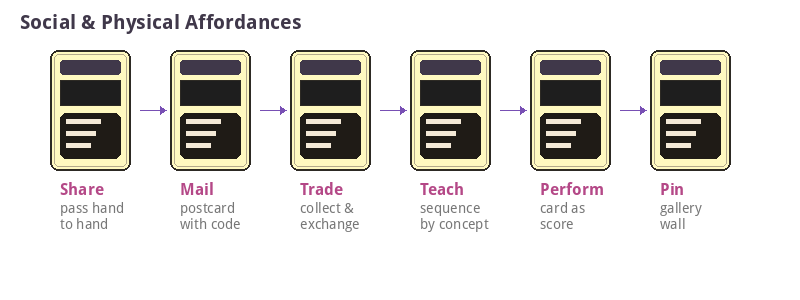
\includegraphics[width=\textwidth]{layout-affordances.png}
\caption{卡片格式的社会和物理可供性。每种可供性源于卡片的物质性：它可以手递手\textbf{分享}，作为明信片\textbf{邮寄}，\textbf{交换}和收藏，在教学序列中\textbf{用于教学}，作为图形乐谱\textbf{演奏}，或\textbf{钉}在画廊墙上。}
\label{fig:affordances}
\end{figure*}

\subsection{卡组编排}

卡片不是单独的物件。它们组成卡组，卡组的编排创造意义。一个\emph{教学序列}按概念排序卡片：先是方块（坐标），然后线条（三角函数），圆形（半径和重复），数学曲线（plot 和正弦），海龟图形（相对运动），最后是公案（极简表达）。一个\emph{画廊网格}在墙上空间排列卡片，邀请跨类别比较。一副\emph{洗牌卡组}随机化顺序，在分形和地平线之间、在树和点之间产生意想不到的并置。

\begin{figure}[h]
\centering
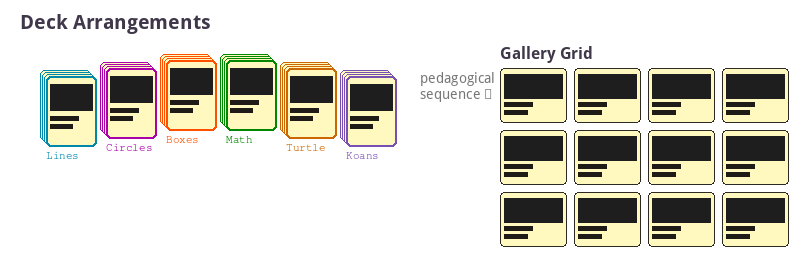
\includegraphics[width=\columnwidth]{layout-decks.png}
\caption{卡组编排。左：按类别展开的卡片（线条、圆形、方块、数学、海龟、公案），每个类别有多张卡片堆叠。右：一个画廊网格，卡片按空间排列供浏览。}
\label{fig:decks}
\end{figure}

% ============ 6. 现实中的卡片 ============

\section{现实中的卡片}
\label{sec:wild}

笔记本卡片是练习。真正的 \kidlisp{} 语料库------59位作者创建的16,000多个程序------包含使用完整运行时的作品：动画、音频、嵌入层、渐变淡出、随机放置和定时语法。这些作品足够短，适合卡片格式，但远比笔记本示例更具表现力。它们的预览图像由 oven 服务（基于 Puppeteer 的屏幕捕获）渲染，并通过 CDN 提供。

\begin{figure*}[t]
\centering
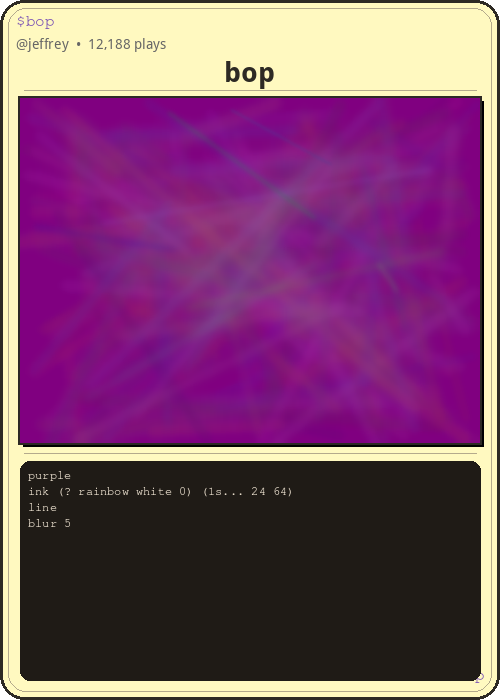
\includegraphics[height=7cm]{user-card-bop.png}%
\hfill%
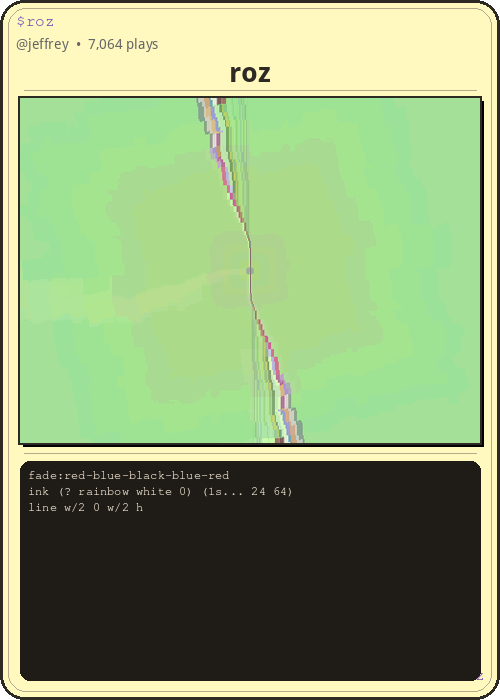
\includegraphics[height=7cm]{user-card-roz.png}%
\hfill%
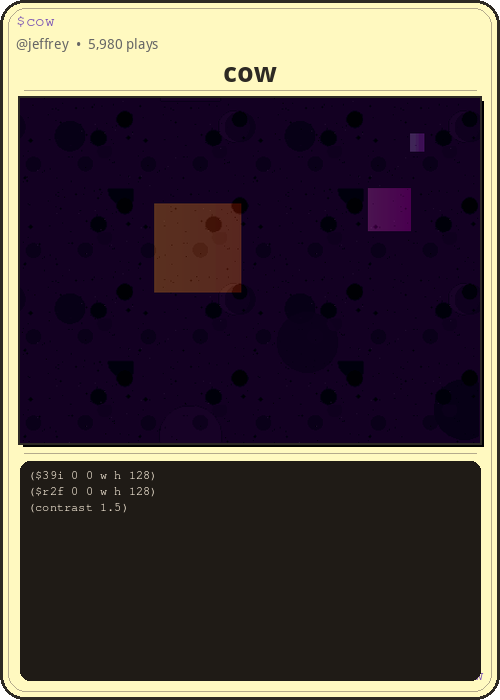
\includegraphics[height=7cm]{user-card-cow.png}%
\hfill%
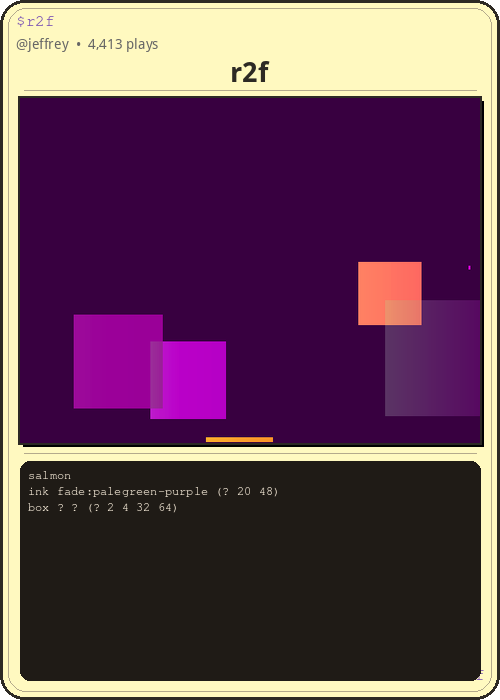
\includegraphics[height=7cm]{user-card-r2f.png}
\caption{来自 \kidlisp{} 活跃语料库的四张卡片，由 oven 服务渲染。从左到右：\texttt{\$bop}（12,188次播放------最受欢迎的作品，4行），\texttt{\$roz}（7,064次播放，3行），\texttt{\$cow}（5,980次播放------通过 \texttt{\$39i} 和 \texttt{\$r2f} 嵌入其他两个作品的组合），\texttt{\$r2f}（4,413次播放，3行随机方块放置）。全部出自 @jeffrey。这些程序使用了 Python 解释器中不存在的功能------动画、随机性（\texttt{?}）、渐变淡出（\texttt{fade:}）、嵌入层（\texttt{\$code}）------但它们的源代码仍然放得下一张卡片。}
\label{fig:user-cards}
\end{figure*}

\subsection{真实作品增添了什么}

笔记本卡片使用 \kidlisp{} 的静态子集。\texttt{kidlisp.com} 上的真实作品使用完整运行时：

\begin{itemize}
  \item \textbf{动画。}程序每帧重新求值。\texttt{frame} 和 \texttt{time} 自动变化。单帧截图捕捉一个活跃作品的一个瞬间。
  \item \textbf{随机性。}\texttt{?} 运算符每帧从列表中产生一个随机值。\texttt{(ink (? red blue green))} 在颜色间闪烁。
  \item \textbf{渐变淡出。}\texttt{fade:red-blue-black} 在画布上插值多停点渐变，由 \texttt{frame} 计数驱动。一个表达式替代了数页手动颜色数学。
  \item \textbf{嵌入。}\texttt{(\$cow)} 从 MongoDB 获取作品 \texttt{cow}，在离屏缓冲区中求值，并合成结果。作品构建于作品之上。
  \item \textbf{定时。}\texttt{1s... (zoom 0.5)} 每秒应用一次缩放。无需显式动画循环。
\end{itemize}

这些功能使程序保持简短，同时极大地扩展了其表达能力。\texttt{\$bop}------播放次数最多的作品，12,188次观看------只有四行：紫色背景、彩虹闪烁的墨水、一条随机线和一个模糊。在卡片上，它看起来像动态绘画的一个冻结瞬间。在浏览器中，它确实是。

\subsection{卡片作为快照}

动画作品的卡片必然是不完整的。它捕捉了一个时间过程的一帧。这种不完整性是格式的一部分：卡片邀请你输入代码，看看它实际做了什么。静态图像是承诺。源代码是兑现。短代码（\texttt{\$bop}）是桥梁------在 \texttt{kidlisp.com} 中输入它，卡片就会活过来。

% ============ 7. 卡片可能成为什么 ============

\section{卡片可能成为什么}
\label{sec:futures}

卡片格式还很年轻。当前笔记本是概念验证------28个离线渲染的程序。但短程序与物理卡片之间的对应关系暗示了几个方向。

\subsection{集换卡}

KidLisp 卡片具有大多数软件所不具备的可收藏性。每张卡片有名称、视觉身份、短代码（\texttt{\$xyz}）和作者。卡片可以印刷、编号和交换。稀有卡片可能使用晦涩的语言特性，或从最少的代码产生意想不到的复杂输出。卡片的"稀有度"就是其信息密度：从多少个字符中涌现出多少视觉复杂性。

\subsection{教学序列}

当前笔记本中的七个类别暗示了一种教学顺序：从方块开始（简单坐标），进而到线条（三角函数）、圆形（半径和重复）、数学曲线（plot 和正弦）、海龟图形（相对运动），最后是公案（极简表达）。每张卡片教授一个概念。教师可以给学生一副实体卡牌，要求他们复现每张卡片、修改它或在同一类别中创建新卡片。

\subsection{印刷乐谱}

在音乐中，乐谱是产生时间事件的指令。KidLisp 卡片是产生视觉事件的指令。卡片可以作为图形乐谱发挥作用，延续 Cornelius Cardew、John Cage 和 Fluxus 事件乐谱的传统。演奏者收到一张卡片，解读代码（在 \texttt{kidlisp.com} 上输入、大声朗读、手绘），然后产生一个事件。卡片就是乐谱。渲染是一种可能的实现。

\subsection{邮寄艺术}

4$\times$6英寸的 KidLisp 卡片就是一张明信片。正面展示渲染图像。背面展示源代码、作者署名和用于在线查找的短代码。带有可执行内容的邮寄艺术------收件人可以输入代码，在自己的屏幕上看到图像重新生成。物理卡片和数字程序是同一作品的两种媒介。

\subsection{生成式文具}

由于 Python 解释器是确定性的且独立运行的，卡片可以在没有网络访问的情况下批量渲染用于印刷制作。一套卡片可以印刷成小册子、独立出版物或盒装套件。\texttt{cards-convert.mjs} 管线已经能从论文格式生成4$\times$6英寸的 PDF 卡片；将其扩展为同时包含渲染的程序输出和源代码是自然的下一步。

\subsection{约束作为生成原则}

卡片格式最有趣的后果是它如何反馈到语言中。放不进卡片的程序暗示着缺失的抽象------或者暗示程序做得太多。卡片约束鼓励经济性：找到产生最有趣图像的三行程序。这是 Oulipo 传统中的生成性约束------任意的形式限制产生意想不到的创造性结果。

% ============ 6. 相关工作 ============

\section{相关工作}

\textbf{印刷代码。}演示场景中的"sizecoding"传统（256字节以下的程序）与最小程序产生最大输出的美学一脉相承。\kidlisp{} 卡片更接近"代码诗"传统，其中源代码本身作为文本与其输出一起被阅读。

\textbf{图形乐谱。}Cardew 的 \emph{Treatise}（1967）和 Cage 的 \emph{Notations}（1969）确立了视觉符号可以作为演奏指令而不规定特定实现。KidLisp 卡片的不同之处在于它们是完全可执行的------渲染是确定性的，不开放解读。但卡片即乐谱的框架邀请重新诠释：如果你每次以不同方式"演奏"卡片会怎样？

\textbf{集换卡游戏。}\emph{Magic: The Gathering}（1993）等游戏证明，具有结构化元数据（名称、类型、规则文本、插图）的卡片创造了丰富的组合空间。KidLisp 卡片具有自然的元数据（标题、类别、函数数量、行数、输出复杂度），可以支持类似的游戏机制。

\textbf{计算笔记本。}Jupyter 笔记本已经将代码和输出结合在一起。KidLisp Cards 笔记本是一个 Jupyter 笔记本，但有一个特定的约束：每个单元格是一张自包含的卡片，而不是更长计算中的一个步骤。笔记本是画廊，不是叙事。

% ============ 7. 结论 ============

\section{结论}

KidLisp 卡片源于一个简单的观察：当程序足够短时，它们就能放在卡片上。卡片格式------标题、图像、源代码------将程序变成可以打印、邮寄、收藏、用于教学和演奏的物理制品。Python 渲染管线实现了离线批量制作。七个类别的目录提供了进入语言的策展入口。

该格式是一项进行中的工作。当前28张卡片的卡组是起点，不是完成的收藏。问题不在于制作多少张卡片，而在于哪些程序值得成为卡片------哪些三行构图产生的图像值得握在手中。

笔记本、解释器和卡片目录可在 \url{https://github.com/whistlegraph/aesthetic-computer} 获取。程序可在 \url{https://kidlisp.com} 上创建和分享。

\vspace{0.5em}
\noindent\textbf{ORCID:} \href{https://orcid.org/0009-0007-4460-4913}{0009-0007-4460-4913}

% ============ 参考文献 ============

\bibliographystyle{plainnat}
\bibliography{references}

\end{document}
